% comment out for student version
\ifdefined\Student\relax\else\def\Teacher{}\fi

\documentclass[12pt]{article}

\title{Linked Structures}
\author{C.~Mayfield, D.~Weikle, and N.~Sprague}
\date{Summer 2021}

%\ProvidesPackage{cspogil}

% fonts
\usepackage[utf8]{inputenc}
\usepackage[T1]{fontenc}
\usepackage{mathpazo}

% spacing
\usepackage[margin=2cm]{geometry}
\renewcommand{\arraystretch}{1.4}
\setlength{\parindent}{0pt}

% orphans and widows
\clubpenalty=10000
\widowpenalty=10000
\pagestyle{empty}

% figures and tables
\usepackage{graphicx}
\usepackage{multicol}
\usepackage{tabularx}
\usepackage{wrapfig}

% fixed-width columns
\usepackage{array}
\newcolumntype{L}[1]{>{\raggedright\let\newline\\\arraybackslash\hspace{0pt}}m{#1}}
\newcolumntype{C}[1]{>{\centering\let\newline\\\arraybackslash\hspace{0pt}}m{#1}}
\newcolumntype{R}[1]{>{\raggedleft\let\newline\\\arraybackslash\hspace{0pt}}m{#1}}

% include paths
\makeatletter
\def\input@path{{Models/}{../../Models/}}
\graphicspath{{Models/}{../../Models/}}
\makeatother

% colors
\usepackage[svgnames,table]{xcolor}
\definecolor{bgcolor}{HTML}{FAFAFA}
\definecolor{comment}{HTML}{007C00}
\definecolor{keyword}{HTML}{0000FF}
\definecolor{strings}{HTML}{B20000}

% table headers
\newcommand{\tr}{\bf\cellcolor{Yellow!10}}

% syntax highlighting
\usepackage{textcomp}
\usepackage{listings}
\lstset{
    basicstyle=\ttfamily\color{black},
    backgroundcolor=\color{bgcolor},
    numberstyle=\scriptsize\color{comment},
    commentstyle=\color{comment},
    keywordstyle=\color{keyword},
    stringstyle=\color{strings},
    columns=fullflexible,
    keepspaces=true,
    showlines=true,
    showstringspaces=false,
    upquote=true
}

% code environments
\newcommand{\java}[1]{\lstinline[language=java]{#1}}%[
\lstnewenvironment{javalst}{\lstset{language=java,backgroundcolor=}}{}
\lstnewenvironment{javabox}{\lstset{language=java,frame=single,numbers=left}\quote}{\endquote}

% PDF properties
\usepackage[pdftex]{hyperref}
\urlstyle{same}
\makeatletter
\hypersetup{
  pdftitle={\@title},
  pdfauthor={\@author},
  pdfsubject={\@date},
  pdfkeywords={},
  bookmarksopen=false,
  colorlinks=true,
  citecolor=black,
  filecolor=black,
  linkcolor=black,
  urlcolor=blue
}
\makeatother

% titles
\makeatletter
\renewcommand{\maketitle}{\begin{center}\LARGE\@title\end{center}}
\makeatother

% boxes [optional height]
\newcommand{\emptybox}[1][10em]{
\vspace{1em}
\begin{tabularx}{\linewidth}{|X|}
\hline\\[#1]\hline
\end{tabularx}}

% models
\newcommand{\model}[1]{\section{#1}\nopagebreak}
\renewcommand{\thesection}{Model~\arabic{section}}

% questions
\newcommand{\quest}[1]{\subsection*{Questions~ (#1)}}
\newcounter{question}
\newcommand{\Q}{\vspace{1em}\refstepcounter{question}\arabic{question}.~ }
\renewcommand{\thequestion}{\#\arabic{question}}

% sub-question lists
\usepackage{enumitem}
\setenumerate[1]{label=\alph*)}
\setlist{itemsep=1em,after=\vspace{1ex}}

% inline answers
\definecolor{answers}{HTML}{C0C0C0}
\newcommand{\ans}[1]{%
\ifdefined\Student
    \leavevmode\phantom{~~\textcolor{answers}{#1}}
\else
    ~~\textcolor{answers}{#1}
\fi}

% longer answers [optional height]
\newsavebox{\ansbox}
\newenvironment{answer}[1][4em]{
\nopagebreak
\begin{lrbox}{\ansbox}
\begin{minipage}[t][#1]{\linewidth}
\color{answers}
}{
\end{minipage}
\end{lrbox}
\ifdefined\Student
    \phantom{\usebox{\ansbox}}%
\else
    \usebox{\ansbox}%
\fi}


\begin{document}

\maketitle

The \textit{Java Collections Framework} provides many useful interfaces and implementations (classes). %, and algorithms (methods).
They all serve the same purpose: to store a collection of objects.
Each type of collection has its trade-offs, and there is no one ``best solution'' for every storage problem.
%If arrays were good enough, Java wouldn't need a collections framework.

%\medskip
%Today you will learn one of the most fundamental concepts of data structures: whether to store elements in contiguous memory locations (arrays), or link elements together using references.

\rolenames

\guide{
  \item Show the contents of a List after adding and removing elements.
  \item Summarize performance trade-offs for ArrayList and LinkedList.
}{
  \item Making connections between list diagrams and source code. (Information Processing)
}{
\ref{list-interface.tex} should be a quick review based on students' prior experience with \java{ArrayList}s.
Report out \ref{listtable} by projecting (or drawing) the table on the board and asking presenters to fill in rows.

Within the first five minutes of \ref{array-lists.tex}, report out on \ref{arrayopers} to make sure students understand what is meant by ``operations'' (assignments).
Note that \ref{linked-lists.tex} continues this idea to include assigning references.
Avoid discussing low-level details such as memory management and object overhead.
After reporting out \ref{ArraysAreBad} and \ref{LinksAreBad}, run one of them for about 10 seconds.
Then terminate the program, change the list type in \java{main}, and rerun the program.

At the end of \ref{linked-lists.tex}, it is helpful to show the \github{CS1/Act18/util}{Java library source code} for List, ArrayList, and LinkedList.
Help students make connections from the models in this activity to their actual implementation in Java.
For example, you can display the private methods of LinkedList and ask presenters to discuss their team's answer to \ref{LinksAreBad}.

Key questions: \ref{key1}, \ref{key2}, and \ref{key3}

Source files: \src{Act22}{ArraysAreBad.java}, \src{Act22}{LinksAreBad.java}
}

% Based on Model 1 of Lists activity by Clif Kussmaul

\model{List Interface}

In computer science, a \textit{list} is a group of items with an \textit{index} (or position) for each item.

\begin{center}
\begin{tabular}{|c|c|c|c|c|c|c|c|c|c|}
\hline
\tr \textbf{index:} & 0 & 1 & 2 & 3 & 4 & 5 & 6 & 7 & \ldots \\
\hline
\tr \textbf{item:} & \str{Mer} & \str{Ven} & \str{Ear} & \str{Mar} & \str{Jup} & \str{Sat} & \str{Ura} & \str{Nep} & \ldots \\
\hline
\end{tabular}
\end{center}

Since we know which item is first, second, etc., we say that the list is \textit{ordered}.
%This does \textbf{not} mean that the items have been sorted in any way.
The first item is at the \textit{head} of the list; the last item is at the \textit{tail} of the list.
Here is a subset of methods from \java{interface List<E>} in the Java API.

\begin{center}
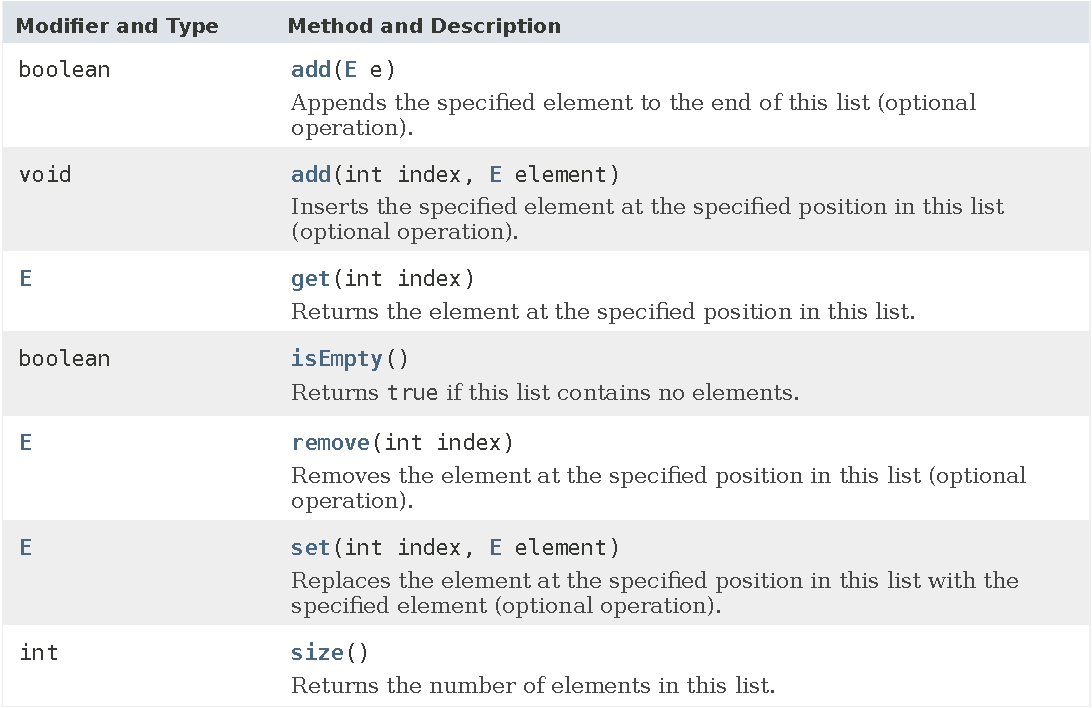
\includegraphics[width=0.85\linewidth]{figs/ListAPI.pdf}
\end{center}


\quest{15 min}


\Q Give several examples of lists from everyday life.

\begin{answer}
Grocery list, playlist on Spotify, to-do lists, etc.
\end{answer}


\Q What is the index of the head of a list?
In general, what is the index of the tail of a list?

\begin{answer}[3em]
The head is at index 0, the tail is at index size - 1.
\end{answer}


\Q In Java lists, what does the \java{<E>} represent?

\begin{answer}
\java{<E>} is a generic type, i.e., the type of the list items.
Notice that \java{add} takes an \java{E} as a parameter, and \java{get} returns an element of type \java{E}.
\end{answer}


\Q Of the seven methods shown from the Java API, how many change the contents of the list?

\begin{answer}[3em]
Four: \java{add} (at the end), \java{add} (at a position), \java{remove}, and \java{set}.
\end{answer}


\Q Fill in the table below using the methods from the Java API.

\vspace{-1ex}
\begin{center}
%TODO need solution (convert table to LaTeX?)
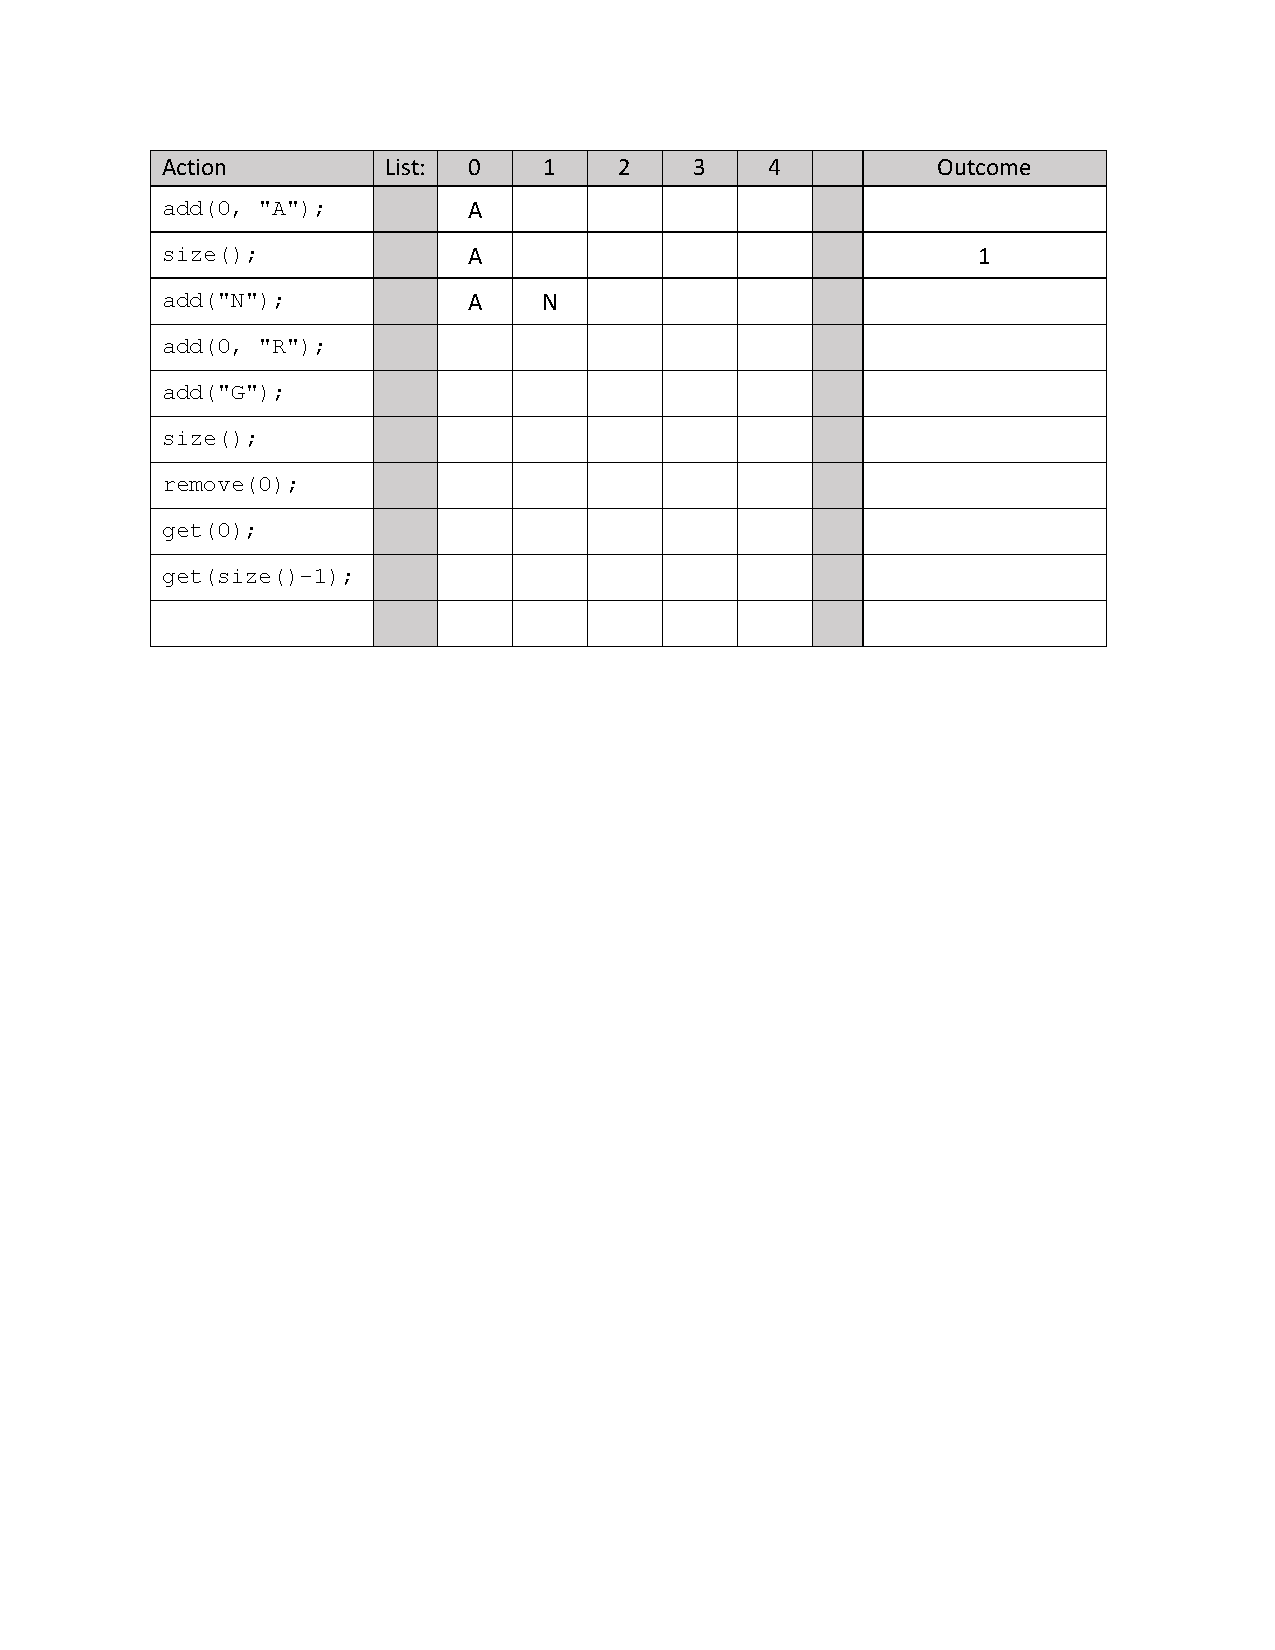
\includegraphics[width=0.85\linewidth]{figs/JavaAPIQuestionTable.pdf}
\end{center}
\vspace{-1ex}


\Q When adding or removing elements at the beginning, what do you have to do with the existing elements in the list?

\begin{answer}
To keep the list in order, existing elements need to be shifted down by one to the right for adding and to the left for removing.
\end{answer}


\Q In your own words, describe what a \java{List} collection is from a programmer's perspective.

\begin{answer}[5em]
A \java{List} is an ordered collection of elements (also known as a sequence).
The user of this interface has precise control over where  each element is inserted.
You can access elements by their integer index and search for elements in the list.
\end{answer}

\newpage
\model{Array Lists}

Arrays store elements in one \emph{contiguous} block of memory.
Since elements are stored together, you can immediately access any element by its index.

\vspace{1ex}
\begin{minipage}{0.50\linewidth}
\begin{javalst}
    int[] numbers = {22, 6, 14};
    System.out.println(numbers[1]);
\end{javalst}
\end{minipage}
\hfill
\begin{minipage}{0.48\linewidth}
\centering
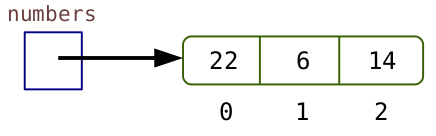
\includegraphics[scale=0.35]{figs/array1.png}
\end{minipage}
\vspace{1ex}

The \java{ArrayList} collection implements \java{List} and uses an array (internally) to store its elements.

\vspace{1ex}
\begin{minipage}{0.35\linewidth}
\begin{javalst}
    ArrayList<Integer> numbers = new ArrayList<>();
    numbers.add(22);
    numbers.add(6);
    numbers.add(14);
\end{javalst}
\end{minipage}
\hfill
\begin{minipage}{0.63\linewidth}
\vspace*{2em}
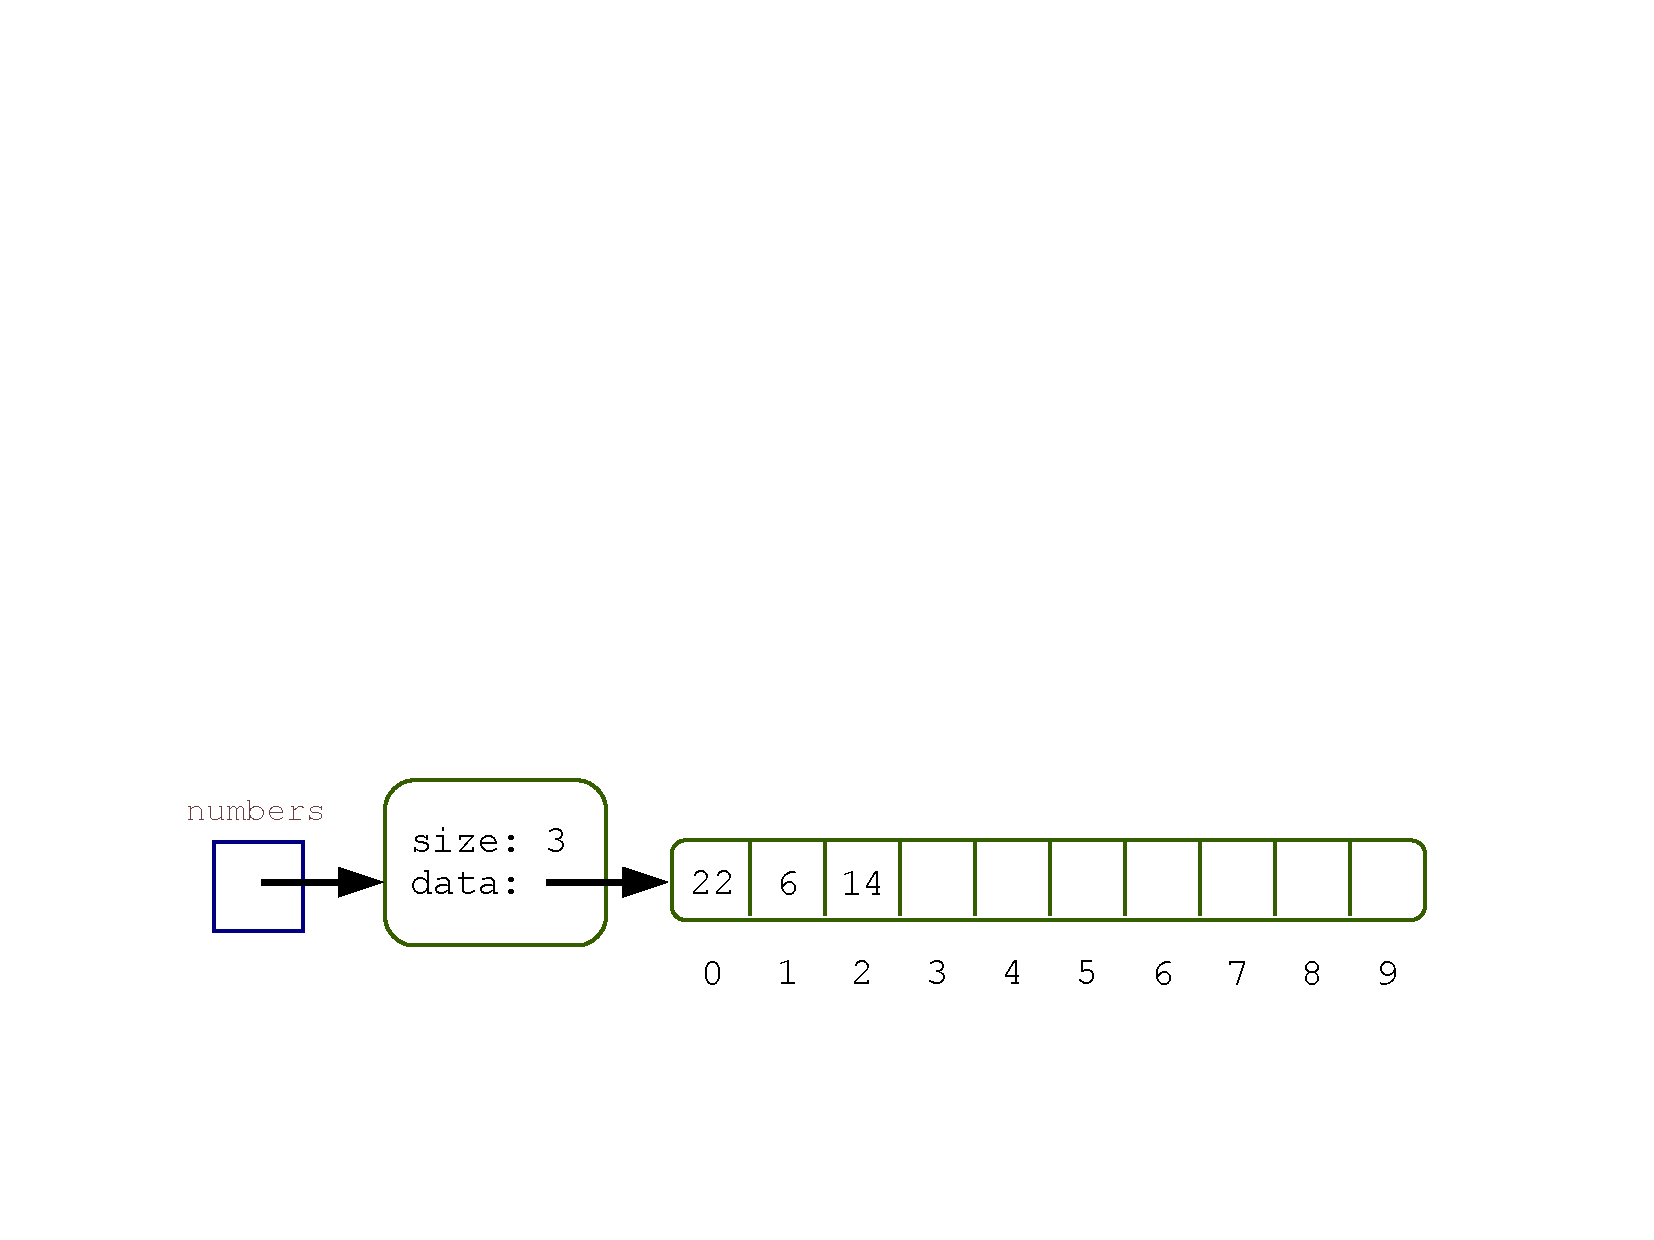
\includegraphics[scale=0.45]{figs/array2.pdf}
%Note these figures have 10 elements because that is the default for an ArrayList
\end{minipage}
\vspace{1ex}

When new values are inserted, existing array elements are moved to the right.

\vspace{1ex}
\begin{minipage}{0.35\linewidth}
\begin{javalst}
    numbers.add(0, 49);
    numbers.add(0, 74);
\end{javalst}
\end{minipage}
\hfill
\begin{minipage}{0.63\linewidth}
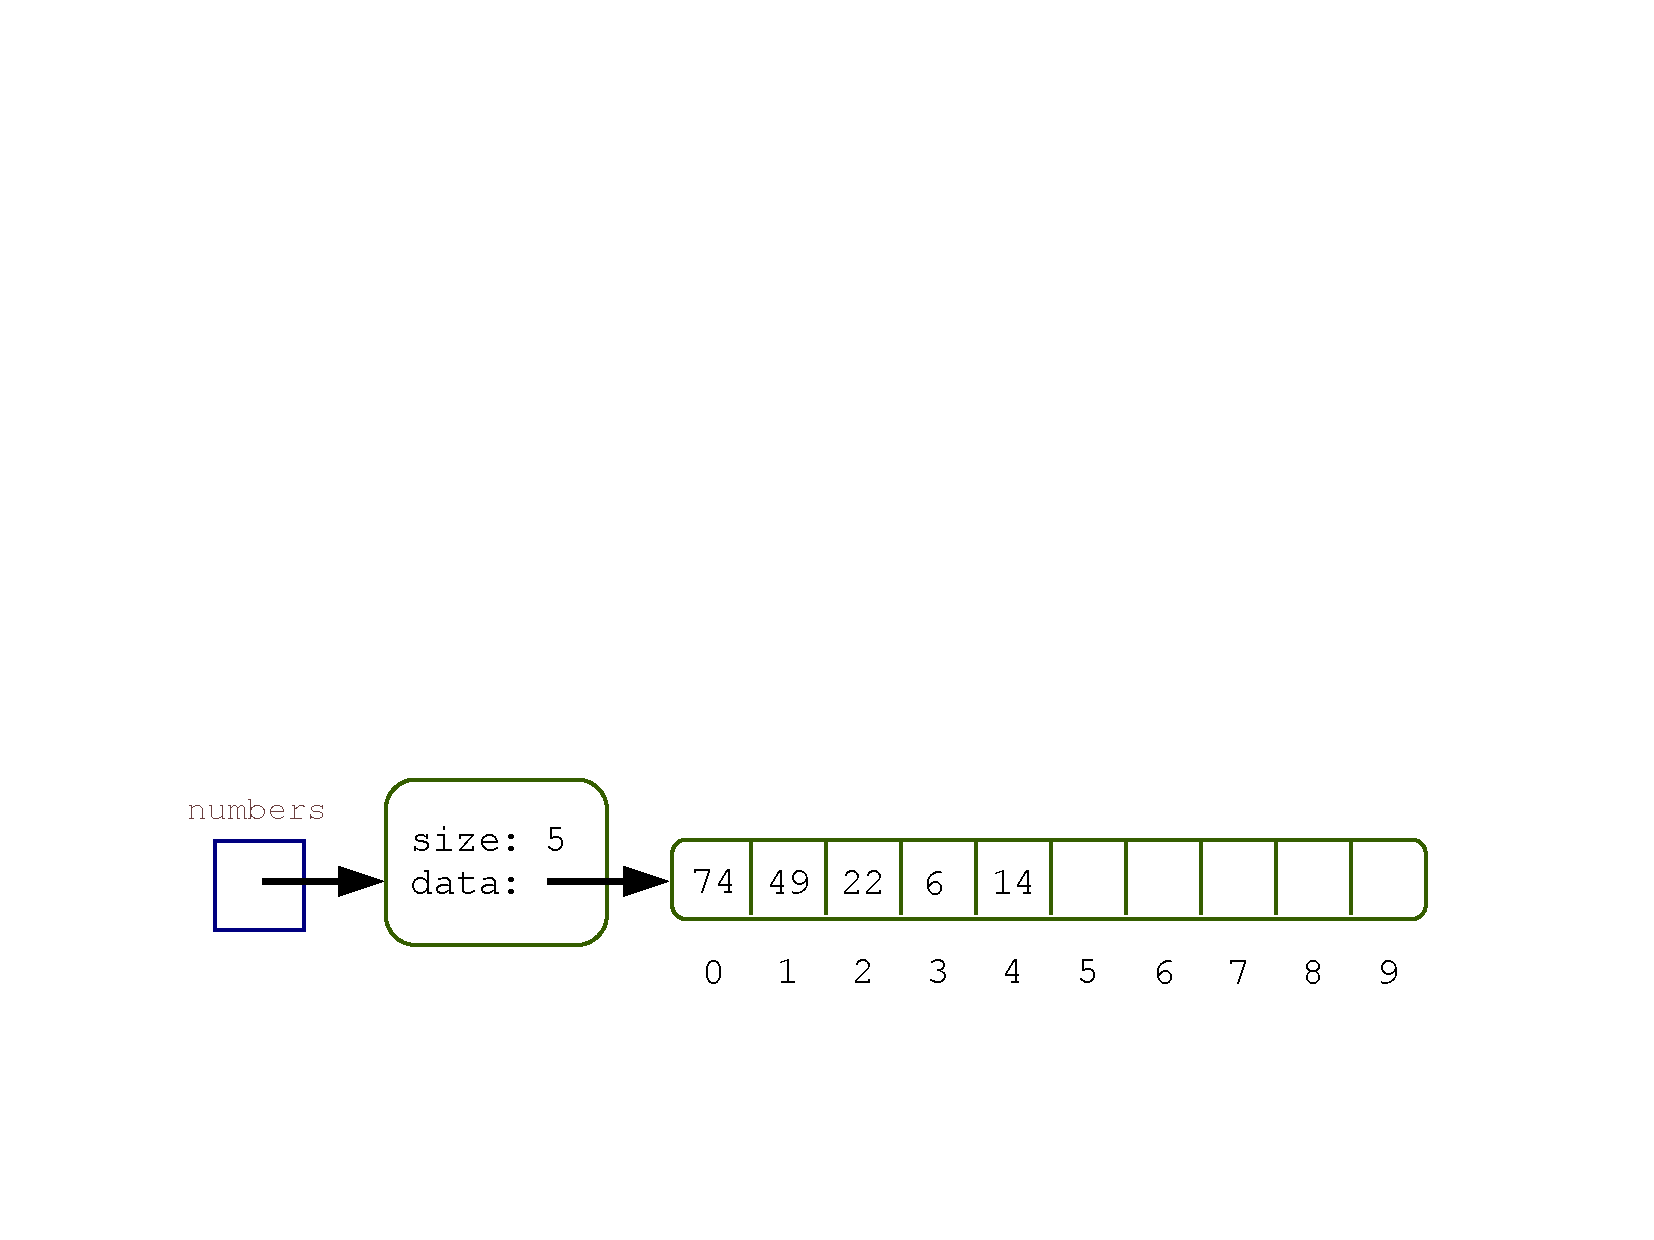
\includegraphics[scale=0.45]{figs/array3.pdf}
\end{minipage}
\vspace{1ex}

If the array fills up, \java{ArrayList} automatically creates a new array about 50\% larger.
All current values must be copied into the new array, and the old array is then garbage collected.


\quest{10 min}


\Q Why does the Java Collections Framework use the name \java{ArrayList}?
(What do the words \java{Array} and \java{List} indicate?)

\begin{answer}
The \java{ArrayList} collection implements the \java{List} interface using an array.
In general, the first word tells how it's implemented, and the second word is the interface.
\end{answer}


%CSM let's not go here; the model hides details of autoboxing
%\Q How much memory is needed for each element in the array?
%
%\begin{answer}
%Each element takes the number of bytes of the size of the element.
%Here it is an Integer object, so 8 bytes for the reference, 16 bytes of object %overhead, and 4 bytes for the actual int.
%\end{answer}


\Q \label{arrayopers}
How many array operations (i.e., integer assignments) were required to add 49 and 79 to the front of the second diagram in \ref{\currfilename}?

\begin{answer}
There are 9 total array operations:
49 takes 4 (3 shifts + 1 add), and 74 takes 5 (4 shifts + 1 add).
\end{answer}


\Q Imagine the internal array for \java{numbers} is full (i.e., with size=10 above).
If you request one more element to be added (at the end), how big will the new array be?

\begin{answer}
50\% of 10 is 5, so the new array will be 15 elements.
\end{answer}


\Q Continuing the previous question, how many operations will it take to add one more element? Briefly describe each operation, beginning with creating the new array.

\begin{answer}
First, a new array of length 15 must be created.
Then, the 10 elements must be copied from the old array to the new array.
Next, the new element is added to the end and the \java{size} attribute is incremented.
Finally, the old array is garbage collected.
\end{answer}


\Q \label{ArraysAreBad}
Discuss why \java{ArrayList} is a poor choice of \java{List} in the program below.

\vspace{1ex}
\begin{javabox}
import java.util.ArrayList;
import java.util.List;

public class ArraysAreBad
{
    public static void main(String[] args)
    {
        ArrayList<String> arrayList = new ArrayList<>();

        System.out.println("ArrayList: ");
        addAndRemoveAtStart(arrayList);
        System.out.println("Done!");
    }

    public static void addAndRemoveAtStart(List<String> list)
    {
        for (int i = 0; i < 1000000; i++)
        {
            list.add(0, "A");  // add at index 0
        }

        for (int i = 0; i < 1000000; i++)
        {
            list.remove(0);  // remove at index 0
        }
    }
}
\end{javabox}
\vspace{-1ex}

\begin{answer}[3em]
Each insertion at the beginning of the array takes $n$ operations (where $n$ is the current size of the collection) in order to shift existing elements down.
\end{answer}


\Q Arrays are simple and effective. Why would we want any other implementation?

\begin{answer}[3em]
They are inefficient when adding and removing items from the beginning (or the middle).
\end{answer}

\newpage
\model{Linked Lists}

Linked structures ``chain'' elements using references.
Each element of the list is called a \emph{node}.

\vspace{1ex}
\begin{minipage}{0.40\linewidth}
\begin{javalst}
    public class Node
    {
        private int value;
        private Node next;
        ...
    }
\end{javalst}
\end{minipage}
\hfill
\begin{minipage}{0.58\linewidth}
\begin{javalst}
    Node node3 = new Node(14, null);
    Node node2 = new Node(6, node3);
    Node numbers = new Node(22, node2);
\end{javalst}
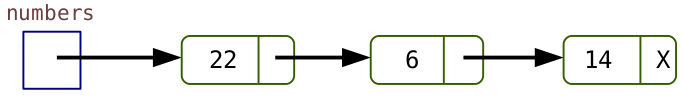
\includegraphics[scale=0.35]{figs/list1.png}
\end{minipage}
\vspace{1em}

This organization allows fast insertions/deletions near the beginning. For example, to add 8:

\vspace{1ex}
\begin{minipage}{0.48\linewidth}
\begin{javalst}
    Node temp = new Node(8, numbers);



    numbers = temp;
\end{javalst}
\end{minipage}
\hfill
\begin{minipage}{0.50\linewidth}
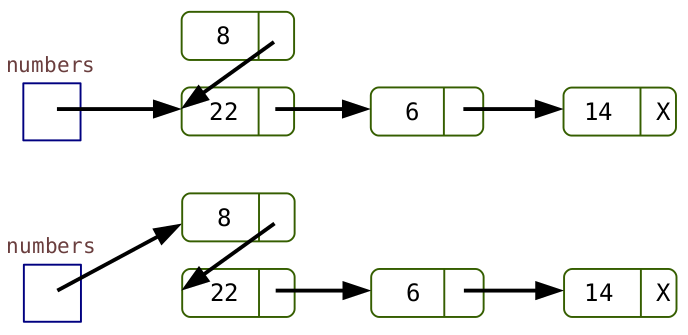
\includegraphics[scale=0.35]{figs/list2.png}
\end{minipage}
\vspace{1em}

Instead of working with nodes directly, we can design a wrapper class to handle list logic:

\vspace{1ex}
\begin{minipage}{0.40\linewidth}
\begin{javalst}
    public class MyList
    {
        private int size;
        private Node head;
        ...
    }
\end{javalst}
\end{minipage}
\hfill
\begin{minipage}{0.58\linewidth}
\begin{javalst}
    MyList numbers = new MyList();
    numbers.addAtStart(14);
    numbers.addAtStart(6);
    numbers.addAtStart(22);
\end{javalst}
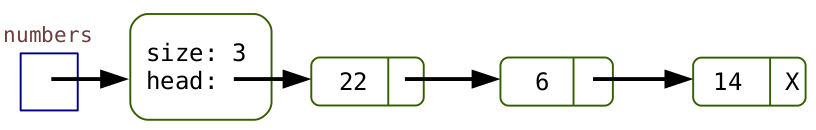
\includegraphics[scale=0.35]{figs/list3.png}
\end{minipage}
\vspace{1ex}


\quest{15 min}


\Q How many assignment operations are required to add 14 {\it at the front} of an empty list? Note that creating a \java{Node} takes two assignments (one for \java{value} and one for \java{next}).

\begin{answer}
3 operations: 1 to assign the \java{value}, 1 to assign null to \java{next}, and 1 to assign the reference of the new Node to the head variable (node3 in this case).
\end{answer}


\Q How many operations are required to add 22 at the front, after 14 and 6 have been added?

\begin{answer}
Still just 3, in fact the same as the first insert. Note that no shifting is required.
\end{answer}


\Q Using this model, how many operations are required to add another element {\it at the end} of the current list?

\begin{answer}[3em]
5 operations: 3 to find where the new element goes (by following references to the end of the list), one to create the new node, and one to change the reference of the previous last element.
\end{answer}


\Q How much memory is needed to store each element in the \java{LinkedList}?
How does that amount compare with using an \java{ArrayList}?

\begin{answer}
Linked lists need to store two references per node (one for \java{value} and one for \java{next}).
In contrast, array lists only need to store the \java{value} references.
At a conceptual level, array lists take up about half as much space as linked lists (not counting empty cells and object overhead).
\end{answer}


\Q \label{LinksAreBad}
Discuss why \java{LinkedList} is a poor choice of \java{List} in the program below.

\vspace{1ex}
\begin{javabox}
import java.util.LinkedList;
import java.util.List;

public class LinksAreBad
{
    public static void main(String[] args)
    {
        LinkedList<String> linkedList = new LinkedList<>();

        System.out.println("LinkedList: ");
        addAndGet(linkedList);
        System.out.println("Done!");
    }

    public static void addAndGet(List<String> list)
    {
        for (int i = 0; i < 1000000; i++)
        {
            list.add("A");  // add at the end
        }

        for (int i = 0; i < 1000000; i++)
        {
            list.get(list.size() / 2);  // get the middle element
        }
    }
}
\end{javabox}
\vspace{-1ex}

\begin{answer}[3em]
Each insertion in the middle of the list takes $n/2$ operations (where $n$ is the current size of the collection) in order to find the \java{next} references to assign.
\end{answer}


\end{document}
